\setcounter{ExampleCounter}{1}
\begin{center}
\includegraphics[width=0.8\textwidth]{tesla_navigation}
\end{center}
How does a navigation system find the best route to the destination?  This is an incredibly complicated problem, searching through all possible routes, each with potentially dozens of twists and turns, to find the best one.  In this section, we'll actually learn the basic process that underlies the way that Google Maps and similar programs use.

To begin, remember that in the first section of this chapter, we discussed \emph{weighted graphs}, like the one below, where each edge has a cost or weight associated with it.  In the context of mapping software, each edge represents a road or street between two intersections, and the weight could represent either the distance between the intersections or the time required to travel along that edge.
\begin{center}
\begin{tikzpicture}[scale=2.5]
  %\GraphInit[vstyle=simple]
  %\tikzset{VertexStyle/.append style={scale=0.5}}
  \Vertex[x=0,y=0]{1}
  \Vertex[x=0,y=2]{2}
  \Vertex[x=0.5,y=1]{3}
  \Vertex[x=2,y=1.8]{4}
  \Vertex[x=1.8,y=-0.1]{5}
  \Vertex[x=2.5,y=0.8]{6}
  \Vertex[x=3.5,y=1.5]{7}
  \Vertex[x=3.4,y=0]{8}
  
  %\tikzstyle{LabelStyle}=[fill=white,sloped]
  \Edge[label=$0.14$](1)(2)
  \Edge[label=$0.63$](2)(3)
  \Edge[label=$0.54$](1)(3)
  \Edge[label=$0.31$](2)(4)
  \Edge[label=$0.35$](3)(4)
  \Edge[label=$0.30$](3)(6)
  \Edge[label=$0.31$](3)(5)
  \Edge[label=$0.47$](1)(5)
  \Edge[label=$0.54$](4)(6)
  \Edge[label=$0.54$](5)(6)
  \Edge[label=$0.43$](4)(7)
  \Edge[label=$0.54$](6)(7)
  \Edge[label=$0.62$](6)(8)
  \Edge[label=$0.37$](7)(8)
\end{tikzpicture}
\end{center}

In other applications, the cost could actually represent cost; for instance, we could draw a travel network where each edge represented a flight between two cities, and the edge weights could be the price of each airline ticket.\\

In this section, we'll address two different questions related to finding the \emph{shortest} path through a graph, meaning the path with the lowest total weight.  For instance, in the graph above, the path $3 \to 4 \to 6 \to 8$ would have a total weight of
\[0.35 + 0.54 + 0.62 = 1.51\]
We call this the \textbf{length} of this path.  Notice that we aren't using length here to refer to the number of edges on the path, and certainly not to the actual drawn length of the lines, since those are arbitrary.

The two questions we'll consider are what we will call here the \textbf{Mail Delivery Problem} and the \textbf{Navigation Problem}.\\

\begin{tabular}{l l}
\parbox[m]{0.15\textwidth}{\includegraphics[width=0.15\textwidth]{usps_truck}}
& \parbox[m]{0.7\textwidth}{In the Mail Delivery Problem, the goal is to \textbf{visit every node} in the graph using the shortest path possible.  This is like a postal worker who must drop off mail in every mailbox along their route, and they would like to do so with as little driving as possible, to save both time and fuel.}
\\
& \\
\parbox[m]{0.15\textwidth}{\includegraphics[width=0.15\textwidth]{phone_navigation}}
& \parbox[m]{0.7\textwidth}{In the Navigation Problem, the goal is to \textbf{get from one point to another} along the shortest route.  In this problem, there's no need to visit every node; the only goal is to get to the destination, again with the lowest possible total cost.}
\end{tabular}\\ \\ \\
The Mail Delivery Problem is also called the Traveling Salesperson Problem, and it is a famous problem in mathematics and computer science.\\

To tackle these problems, we'll learn about two \emph{algorithms}:\marginnote{An \textbf{algorithm} is simply a process, or set of steps, used to accomplish a goal; an algorithm can be thought of as a recipe.  For instance, long division is an algorithm used to divide two numbers.  In most algorithms, there is some repetition or cycling; you can see this if you use long division.\\ \text{}\\

Algorithms are a common topic in computer science (which is one of the fields that uses graph theory the most); most programs can be called algorithms, in the sense that they describe a sequence of commands for the computer to follow.}
\begin{enumerate}
\item To solve the Mail Delivery Problem, we'll use the \textbf{Nearest Neighbor Algorithm}
\item For the Navigation Problem, we'll use \textbf{Dijkstra's Algorithm}, named for a Dutch computer scientist.
\end{enumerate}

\subsection{Mail Delivery - The Nearest Neighbor Algorithm}
The most straightforward way to approach this problem of visiting every node with the shortest path is to check all the possibilities.  Let's use the example of 5 cities in Maryland: Frederick, Baltimore, Annapolis, Columbia, and Rockville.  For simplicity, we'll use the straight-line distance between them, shown on the graph below in miles.

\begin{center}
\begin{tikzpicture}[scale=2.5]
  \GraphInit[vstyle=simple]
  \tikzset{VertexStyle/.append style={scale=0.5}}
  \Vertex[x=0,y=0]{Frederick}
  \Vertex[x=3.2,y=-0.6]{Baltimore}
  \Vertex[x=3.5,y=-2]{Annapolis}
  \Vertex[x=2,y=-0.7]{Columbia}
  \Vertex[x=0.6,y=-1.7]{Rockville}
  
  \extralabel[2mm]{Frederick}{90}{Frederick}
  \extralabel[2mm]{Baltimore}{90}{Baltimore}
  \extralabel[2mm]{Annapolis}{-90}{Annapolis}
  \extralabel[2mm]{Columbia}{90}{Columbia}
  \extralabel[2mm]{Rockville}{-90}{Rockville}
  
  \Edge[label=$45$](Frederick)(Baltimore)
  \Edge[label=$34$](Frederick)(Columbia)
  \Edge[label=$28$](Frederick)(Rockville)
  \Edge[label=$14$](Baltimore)(Columbia)
  \Edge[label=$21$](Baltimore)(Annapolis)
  \Edge[label=$19$](Columbia)(Rockville)
  \Edge[label=$24$](Columbia)(Annapolis)
  \Edge[label=$35$](Rockville)(Annapolis)
  \tikzstyle{LabelStyle}=[fill=white,pos=0.3]
  \Edge[label=$34$](Rockville)(Baltimore)
  \Edge[label=$57$](Frederick)(Annapolis)
\end{tikzpicture}
\end{center}

Instead of this graph, we could also use a table like the following one to show the distances between all the cities:
\begin{center}
\begin{tabular}{l | c c c c c}
& Frederick & Baltimore & Annapolis & Columbia & Rockville\\
\hline
Frederick & -- & 45 & 57 & 34 & 28\\
Baltimore & 45 & -- & 21 & 14 & 34\\
Annapolis & 57 & 21 & -- & 24 & 35\\
Columbia & 34 & 14 & 24 & -- & 19\\
Rockville & 28 & 34 & 35 & 19 & --
\end{tabular}
\end{center}
In order to read this table to find the distance between two cities, locate the column for one city and the row for the other city, and the distance is at the intersection (the dashes represent no distance).  Notice the symmetry in the table: the distance between Frederick and Baltimore is the same as the distance between Baltimore and Frederick.\\
\pagebreak

Now, notice that this is a complete graph, meaning that we can travel from any city to any other.  This is realistic for a mail delivery van or salesperson, but it means that there are many possible paths.  In fact, ignoring reverse paths (meaning that we'll treat Frederick $\to$ Baltimore $\to$ Columbia and Columbia $\to$ Baltimore $\to$ Frederick as the same route), there are a total of 12 ways to travel through this network from any given city.

Let's assume we start and end in Frederick; here are the 12 possible circuits, with the total distance listed for each (abbreviating each city with the first letter of its name):
\begin{center}
\begin{tabular}{c c}
\textbf{Route} & \textbf{Total Distance (miles)}\\
\hline
& \\
$F \to B \to A \to R \to C \to F$ & 154\\
$F \to B \to A \to C \to R \to F$ & 137\\
$F \to B \to C \to R \to A \to F$ & 170\\
$F \to B \to C \to A \to R \to F$ & 146\\
$F \to B \to R \to C \to A \to F$ & 179\\
$F \to B \to R \to A \to C \to F$ & 172\\
$F \to R \to B \to A \to C \to F$ & 141\\
$F \to R \to B \to C \to A \to F$ & 157\\
$F \to R \to C \to B \to A \to F$ & 139\\
$F \to R \to A \to B \to C \to F$ & 132\\
$F \to A \to R \to B \to C \to F$ & 174\\
$F \to A \to B \to R \to C \to F$ & 165\\
\end{tabular}
\end{center}

The shortest possible path is near the bottom of the list: traveling along the route Frederick $\to$ Rockville $\to$ Annapolis $\to$ Baltimore $\to$ Columbia $\to$ Frederick is the best option, for a total distance of 132 miles (47 miles shorter than the worst case).\\

Now, the obvious downside of this method is that it is incredibly tedious to do.  The more serious problem is that as the number of cities increases, the number of possible paths explodes, making this brute-force approach impractical.  For instance, if we used 25 cities (a small number for a local mail delivery), there would be so many possibilities that if we could check one path every nanosecond, it would take about ten million years to find the lengths of all of them.  Since we don't have that kind of time, we need another approach, and for that, we turn to the \textbf{nearest neighbor algorithm}.

\begin{formula}{Nearest Neighbor Algorithm}
At each step, go to the nearest \emph{unvisited} node.  Repeat until all nodes have been visited.\\

This does not generally give the best result, but it is an easy way to get close.
\end{formula}

The nearest neighbor algorithm is an example of a \emph{greedy algorithm}, meaning that it takes the best option at each step without taking a larger view into account.

\def\tryit1graph{\marginnote{\begin{center}
\begin{tikzpicture}[scale=0.75]
  \GraphInit[vstyle=simple]
  \tikzset{VertexStyle/.append style={scale=0.5}}
  \grEmptyCycle[prefix=a,RA=2,rotation=18]{5}
  
  \extralabel{a0}{0}{$b$}
  \extralabel{a1}{90}{$a$}
  \extralabel{a2}{180}{$e$}
  \extralabel{a3}{-90}{$d$}
  \extralabel{a4}{-90}{$c$}
  
  \Edge[label=7](a0)(a1)
  \Edge[label=8](a0)(a2)
  \Edge[label=13](a0)(a3)
  \Edge[label=6](a0)(a4)
  \Edge[label=5](a1)(a2)
  \Edge[label=11](a1)(a3)
  \Edge[label=3](a1)(a4)
  \Edge[label=12](a2)(a3)
  \Edge[label=9](a2)(a4)
  \Edge[label=10](a3)(a4)
\end{tikzpicture}
\end{center}}}

\begin{example}{Nearest Neighbor Algorithm}
Use the nearest neighbor algorithm to find a possible minimum circuit through the Maryland cities, starting and ending at Frederick.

\sol
Starting at Frederick, the closest city is Rockville.  Once we get to Rockville, the closest city (besides Frederick, since we've already been there), is Columbia, so we go there.  From there, Baltimore is the closest remaining city, which just leaves Annapolis before we return to Frederick:
\begin{center}
Circuit: $\boxed{F \to R \to C \to B \to A \to F}$
\end{center}

The\tryit1graph total distance is 139 miles; notice that while this isn't the best possible path, it \emph{is} the third best, only 7 miles longer than the optimal one.  And the advantage is obvious; this process was much quicker and simpler than the brute force approach.
\end{example}

\begin{trynolabel}
Using the graph shown in the margin, use the nearest neighbor algorithm to find a possible minimum circuit starting at $a$, then repeat this starting at $b$ and starting at $c$.
\end{trynolabel}
\pagebreak

\subsection{Navigation - Dijkstra's Algorithm}
Edsger Dijkstra\marginnote{\includegraphics[width=1.5in]{edsgerdijkstra}\\Edsger Dijkstra in 2002\\{\tiny\color{gray} CC BY-SA 3.0, Hamilton Richards}} (\emph{pronounced DIKE-stra}) was a Dutch computer scientist before there was such a thing (before there were computer scientists, that is, not before there were Dutch people).  In the 1950s, when he got married, he was required to put his profession on the application for a marriage license, and when he wrote ``programmer,'' the authorities made him change it, since there was no such profession.  Instead, he stated that he was a theoretical physicist, which was his first course of study.

Dijkstra was brilliant, and he went on to lay much of the foundation for modern computer science.  One of the problems studied was this problem of navigation, finding the shortest path between two points on a graph.  His solution has been applied to many fields, including robotics (navigating a robot around obstacles), transportation, and even games (finding an optimal solution for a Rubik's cube).\\

Dijkstra's algorithm is more complicated than the nearest neighbor algorithm, at least at first.  The actual steps, though, are very simple mathematically.  Before we give the full algorithm, let's do a simple example to illustrate how it works.  Start with the graph below:
\begin{center}
\begin{tikzpicture}
  \GraphInit[vstyle=simple]
  \tikzset{VertexStyle/.append style={scale=0.3}}
  \SetGraphUnit{1.1}
  
  \Vertex{a}
  \NOEA(a){b}
  \EA(b){c}
  \SOEA(c){d}
  \SOWE(d){e}
  \WE(e){f}
  
  \extralabel{a}{180}{$a$}
  \extralabel{b}{90}{$b$}
  \extralabel{c}{90}{$c$}
  \extralabel{d}{0}{$d$}
  \extralabel{e}{-90}{$e$}
  \extralabel{f}{-90}{$f$}
  
  \Edge[label=4](a)(b)
  \Edge[label=3](a)(f)
  \Edge[label=5](c)(f)
  \Edge[label=2](e)(d)
  \Edge[label=3](c)(d)
  \Edge[label=2](b)(c)
  \Edge[label=3](e)(f)
\end{tikzpicture}
\end{center}

\def\shortestpathexa{\marginnote{\begin{center}
\begin{tikzpicture}
  \GraphInit[vstyle=simple]
  \tikzset{VertexStyle/.append style={scale=0.3}}
  \SetGraphUnit{0.85}
  
  \Vertex{a}
  \NOEA(a){b}
  \EA(b){c}
  \SOEA(c){d}
  \SOWE(d){e}
  \WE(e){f}
  
  \extralabel{a}{180}{$a$}
  \extralabel{b}{90}{$b$}
  \extralabel{c}{90}{$c$}
  \extralabel{d}{0}{$d$}
  \extralabel{e}{-90}{$e$}
  \extralabel{f}{-90}{$f$}
  \extralabel{b}{135}{\color{red}\circled{4}}
  \extralabel{f}{225}{\color{red}\circled{3}}
  
  \Edge[label=4](a)(b)
  \Edge[label=3](a)(f)
  \Edge[label=5](c)(f)
  \Edge[label=2](e)(d)
  \Edge[label=3](c)(d)
  \Edge[label=2](b)(c)
  \Edge[label=3](e)(f)
\end{tikzpicture}
\end{center}}}
\def\shortestpathexb{\marginnote{\begin{center}
\begin{tikzpicture}
  \GraphInit[vstyle=simple]
  \tikzset{VertexStyle/.append style={scale=0.3}}
  \SetGraphUnit{0.85}
  
  \Vertex{a}
  \NOEA(a){b}
  \EA(b){c}
  \SOEA(c){d}
  \SOWE(d){e}
  \WE(e){f}
  
  \extralabel{a}{180}{$a$}
  \extralabel{b}{90}{$b$}
  \extralabel{c}{90}{$c$}
  \extralabel{d}{0}{$d$}
  \extralabel{e}{-90}{$e$}
  \extralabel{f}{-90}{$f$}
  \extralabel{b}{135}{\circled{4}}
  \extralabel{f}{225}{\circled{3}}
  \extralabel{e}{-45}{\color{red}\circled{6}}
  
  \Edge[label=4](a)(b)
  \Edge[label=3](a)(f)
  \Edge[label=5](c)(f)
  \Edge[label=2](e)(d)
  \Edge[label=3](c)(d)
  \Edge[label=2](b)(c)
  \Edge[label=3](e)(f)
\end{tikzpicture}
\end{center}}}
\def\shortestpathexc{\marginnote{\begin{center}
\begin{tikzpicture}
  \GraphInit[vstyle=simple]
  \tikzset{VertexStyle/.append style={scale=0.3}}
  \SetGraphUnit{0.85}
  
  \Vertex{a}
  \NOEA(a){b}
  \EA(b){c}
  \SOEA(c){d}
  \SOWE(d){e}
  \WE(e){f}
  
  \extralabel{a}{180}{$a$}
  \extralabel{b}{90}{$b$}
  \extralabel{c}{90}{$c$}
  \extralabel{d}{0}{$d$}
  \extralabel{e}{-90}{$e$}
  \extralabel{f}{-90}{$f$}
  \extralabel{b}{135}{\circled{4}}
  \extralabel{f}{225}{\circled{3}}
  \extralabel{e}{-45}{\circled{6}}
  \extralabel{c}{45}{\color{red}\circled{6}}
  
  \Edge[label=4](a)(b)
  \Edge[label=3](a)(f)
  \Edge[label=5](c)(f)
  \Edge[label=2](e)(d)
  \Edge[label=3](c)(d)
  \Edge[label=2](b)(c)
  \Edge[label=3](e)(f)
\end{tikzpicture}
\end{center}}}

Now, suppose we want to travel from $a$ to $d$.  This graph is simple enough that we could probably spot the shortest path just by looking at it, but let's illustrate a more systematic process.

Essentially, what the process will do is find the minimum distance (and shortest path) from $a$ to every other point, so once we're done, we just look at the result for $d$.  As we go, we'll keep track of the shortest path to a particular point, and use that to move forward one more step.  For instance,\shortestpathexa\ once we know the shortest path to $c$, we know that we can find the shortest path to $d$ that passes through $c$ by adding 3 for the path from $c$ to $d$.

If we start at $a$, we have two options: go to $b$ (4) or to $f$ (3).  We can keep track of these in a table like this:
\begin{center}
\begin{tabular}{c c l}
\textbf{Node} & \textbf{Minimum Distance from $a$} & \textbf{Shortest Path from $a$}\\
\hline
& & \\
$b$ & 4 & $a \to b$\\
$f$ & 3 & $a \to f$
\end{tabular}
\end{center}

Now, if we take another step, we can get to $c$ (through either $b$ or $f$) and $e$ (through $f$).  Since there's only one option for $e$, let's start there: we can go through $f$ (at a cost of 3) and on to $e$ (another 3) for a total cost of $6$.  Let's add that to the table:\shortestpathexb
\begin{center}
\begin{tabular}{c c l}
\textbf{Node} & \textbf{Minimum Distance from $a$} & \textbf{Shortest Path from $a$}\\
\hline
& & \\
$b$ & 4 & $a \to b$\\
{\LARGE\bfseries\color{red} \emph{e}} & {\Large\bfseries\color{red} 6} & {\LARGE\bfseries\color{red} $a \to f \to e$}\\
$f$ & 3 & $a \to f$
\end{tabular}
\end{center}

For $c$, we have two options: (1) go through $b$, with a total cost of 6 (the 4 to get to $b$, plus the 2 to go from $b$ to $c$), or (2) go through $f$, with a total cost of 8.  Of these, we choose the first option, since it has a lower cost; add that to the table:
\begin{center}
\begin{tabular}{c c l}
\textbf{Node}\shortestpathexc & \textbf{Minimum Distance from $a$} & \textbf{Shortest Path from $a$}\\
\hline
& & \\
$b$ & 4 & $a \to b$\\
{\LARGE\bfseries\color{red} \emph{c}} & {\Large\bfseries\color{red} 6} & {\LARGE\bfseries\color{red} $a \to b \to c$}\\
$e$ & 6 & $a \to f \to e$\\
$f$ & 3 & $a \to f$
\end{tabular}
\end{center}

Our last step ended at either $c$ or $e$, so one more step from either of them will take us to $d$.  Since both are at a minimum distance of 6 from $a$, the best path to $d$ will be the one going through $e$, since that only requires adding 2 to get to $d$, instead of the 3 required from $c$.  Thus, the optimal path from $a$ to $d$ is
\[\boxed{a \to f \to e \to d}\]
which covers a total distance of 8.
\pagebreak

When we actually state Dijkstra's algorithm, it is written in a slightly different form, but the process is what we just outlined: by keeping track of the shortest path from the starting point to all the intermediate nodes, we can move through the graph in waves, so we don't have to evaluate all possible paths.

\begin{formula}{Dijkstra's Algorithm}
To find the shortest path from the origin to the destination:
\begin{enumerate}
\item First, set the initial distances (from the origin) for every node:
\begin{itemize}
\item The distance at the origin is 0.
\item All other distances are infinity ($\infty$) to begin (so that when we find the first real distance, it will be smaller, and we can update this value).
\end{itemize}

\item Next, pick the node (from the ones that we haven't evaluated yet) with the smallest current distance:
\begin{itemize}
\item Update the distances to all its neighbors; if the new distance is shorter than the previous one, replace the old with the new.
\item Check off that node.
\end{itemize}

\item Repeat step 2 until you reach the destination.
\end{enumerate}
\end{formula}

\def\shortestpathexd{\marginnote{\begin{center}
\begin{tikzpicture}[scale=0.7]
  \GraphInit[vstyle=simple]
  \tikzset{VertexStyle/.append style={scale=0.3}}
  \grEmptyCycle[prefix=a,RA=2,rotation=18]{5}
  \grEmptyCycle[prefix=b,RA=0]{1}
  
  \extralabel{a2}{180}{$a$}
  \extralabel{a1}{90}{$b$}
  \extralabel{a0}{0}{$c$}
  \extralabel{a4}{-90}{$d$}
  \extralabel{a3}{-90}{$e$}
  \extralabel{b0}{45}{$f$}
  \extralabel{a1}{135}{\color{red}\circled{14}}
  \extralabel{a3}{225}{\color{red}\circled{7}}
  \extralabel{b0}{0}{\color{red}\circled{9}}
  
  \Edge[label=14](a2)(a1)
  \Edge[label=7](a2)(a3)
  \Edge[label=9](a2)(b0)
  \Edge[label=9](a1)(a0)
  \Edge[label=2](a1)(b0)
  \Edge[label=6](a0)(a4)
  \Edge[label=15](a4)(a3)
  \Edge[label=11](a4)(b0)
  \Edge[label=10](a3)(b0)
\end{tikzpicture}
\end{center}}}
\def\shortestpathexe{\marginnote{\begin{center}
\begin{tikzpicture}[scale=0.7]
  \GraphInit[vstyle=simple]
  \tikzset{VertexStyle/.append style={scale=0.3}}
  \grEmptyCycle[prefix=a,RA=2,rotation=18]{5}
  \grEmptyCycle[prefix=b,RA=0]{1}
  
  \extralabel{a2}{180}{$a$}
  \extralabel{a1}{90}{$b$}
  \extralabel{a0}{0}{$c$}
  \extralabel{a4}{-90}{$d$}
  \extralabel{a3}{-90}{$e$}
  \extralabel{b0}{45}{$f$}
  \extralabel{a1}{135}{\circled{14}}
  \extralabel{a3}{225}{\circled{7}}
  \extralabel{b0}{0}{\circled{9}}
  \extralabel{a4}{225}{\color{red}\circled{22}}
  
  \Edge[label=14](a2)(a1)
  \Edge[label=7](a2)(a3)
  \Edge[label=9](a2)(b0)
  \Edge[label=9](a1)(a0)
  \Edge[label=2](a1)(b0)
  \Edge[label=6](a0)(a4)
  \Edge[label=15](a4)(a3)
  \Edge[label=11](a4)(b0)
  \Edge[label=10](a3)(b0)
\end{tikzpicture}
\end{center}}}
\def\shortestpathexf{\marginnote{\begin{center}
\begin{tikzpicture}[scale=0.7]
  \GraphInit[vstyle=simple]
  \tikzset{VertexStyle/.append style={scale=0.3}}
  \grEmptyCycle[prefix=a,RA=2,rotation=18]{5}
  \grEmptyCycle[prefix=b,RA=0]{1}
  
  \extralabel{a2}{180}{$a$}
  \extralabel{a1}{90}{$b$}
  \extralabel{a0}{0}{$c$}
  \extralabel{a4}{-90}{$d$}
  \extralabel{a3}{-90}{$e$}
  \extralabel{b0}{45}{$f$}
  \extralabel{a1}{135}{\cancel{\circled{14}}}
  \extralabel{a3}{225}{\circled{7}}
  \extralabel{b0}{0}{\circled{9}}
  \extralabel{a4}{225}{\cancel{\circled{22}}}
  \extralabel{a1}{45}{\color{red}\circled{11}}
  \extralabel{a4}{0}{\color{red}\circled{20}}
  
  \Edge[label=14](a2)(a1)
  \Edge[label=7](a2)(a3)
  \Edge[label=9](a2)(b0)
  \Edge[label=9](a1)(a0)
  \Edge[label=2](a1)(b0)
  \Edge[label=6](a0)(a4)
  \Edge[label=15](a4)(a3)
  \Edge[label=11](a4)(b0)
  \Edge[label=10](a3)(b0)
\end{tikzpicture}
\end{center}}}
\def\shortestpathexg{\marginnote{\begin{center}
\begin{tikzpicture}[scale=0.7]
  \GraphInit[vstyle=simple]
  \tikzset{VertexStyle/.append style={scale=0.3}}
  \grEmptyCycle[prefix=a,RA=2,rotation=18]{5}
  \grEmptyCycle[prefix=b,RA=0]{1}
  
  \extralabel{a2}{180}{$a$}
  \extralabel{a1}{90}{$b$}
  \extralabel{a0}{0}{$c$}
  \extralabel{a4}{-90}{$d$}
  \extralabel{a3}{-90}{$e$}
  \extralabel{b0}{45}{$f$}
  \extralabel{a3}{225}{\circled{7}}
  \extralabel{b0}{0}{\circled{9}}
  \extralabel{a1}{45}{\circled{11}}
  \extralabel{a4}{0}{\circled{20}}
  \extralabel{a0}{45}{\color{red}\circled{20}}
  
  \Edge[label=14](a2)(a1)
  \Edge[label=7](a2)(a3)
  \Edge[label=9](a2)(b0)
  \Edge[label=9](a1)(a0)
  \Edge[label=2](a1)(b0)
  \Edge[label=6](a0)(a4)
  \Edge[label=15](a4)(a3)
  \Edge[label=11](a4)(b0)
  \Edge[label=10](a3)(b0)
\end{tikzpicture}
\end{center}}}

\begin{example}{Dijkstra's Algorithm}
Use Dijkstra's algorithm to find the shortest path between $a$ and $c$ in the graph shown below.
\begin{center}
\begin{tikzpicture}
  \GraphInit[vstyle=simple]
  \tikzset{VertexStyle/.append style={scale=0.3}}
  \grEmptyCycle[prefix=a,RA=2,rotation=18]{5}
  \grEmptyCycle[prefix=b,RA=0]{1}
  
  \extralabel{a2}{180}{$a$}
  \extralabel{a1}{90}{$b$}
  \extralabel{a0}{0}{$c$}
  \extralabel{a4}{-90}{$d$}
  \extralabel{a3}{-90}{$e$}
  \extralabel{b0}{30}{$f$}
  
  \Edge[label=14](a2)(a1)
  \Edge[label=7](a2)(a3)
  \Edge[label=9](a2)(b0)
  \Edge[label=9](a1)(a0)
  \Edge[label=2](a1)(b0)
  \Edge[label=6](a0)(a4)
  \Edge[label=15](a4)(a3)
  \Edge[label=11](a4)(b0)
  \Edge[label=10](a3)(b0)
\end{tikzpicture}
\end{center}

\sol
To keep track of the distances, we'll build a table, and update it at every step.  First, we set the initial distances for each point (0 at $a$, infinity everywhere else).
\begin{center}
\begin{tabular}{c c c l}
\textbf{Checked?} & \textbf{Node} & \textbf{Minimum Distance from $a$} & \textbf{Shortest Path from $a$}\\
\hline
& & \\
& $a$ & 0 & \\
& $b$ & $\infty$ & \\
& $c$ & $\infty$ & \\
& $d$ & $\infty$ & \\
& $e$ & $\infty$ & \\
& $f$ & $\infty$ & \\
\end{tabular}
\end{center}

Next, we select the point with the smallest current distance--that would be $a$--and update the distance to all its neighbors.  Since $a$ has $b$, $e$, and $f$ as neighbors, we will update the distance and path for each of these three.  The distance will be the current distance at $a$ (0) plus the distance to the new point, and the path will be the path to $a$ (nothing) with the new segment added on.  Once we do all that, we can check off $a$.
\begin{center}
\begin{tabular}{c c c l}
\textbf{Checked?}\shortestpathexd & \textbf{Node} & \textbf{Min. Distance from $a$} & \textbf{Shortest Path from $a$}\\
\hline
& & \\
\checkmark & $a$ & 0 &\\
& $b$ & $\cancel\infty$\ \ {\color{red}\Large\bfseries 14} & $a \to b$\\
& $c$ & $\infty$ & \\
& $d$ & $\infty$ & \\
& $e$ & $\cancel\infty$\ \ {\color{red}\Large\bfseries 7} & $a \to e$\\
& $f$ & $\cancel\infty$\ \ {\color{red}\Large\bfseries 9} & $a \to f$\\
\end{tabular}
\end{center}

Now we simply repeat this process: select the unchecked point with the smallest distance--which is now $e$--and update its neighbors, then check it off.  By the time we get to $c$, we will be guaranteed to have found the shortest path from $a$ to $c$.\\

The (unchecked) neighbors of $e$ are $d$ and $f$, so for each of them, add the distance to that point from $e$ together with the current distance at $e$ (7).  If that is smaller than the current distance at that point, update the distance and path; if not, do nothing there.\\

For $d$, this results in a distance of $7 + 15 = 22$, which is smaller than $\infty$.  For $f$, however, this gives a distance of $7 + 10 = 17$, which is larger than the current distance there, so we'll leave the row for $f$ unchanged.
\begin{center}
\begin{tabular}{c c c l}
\textbf{Checked?}\shortestpathexe & \textbf{Node} & \textbf{Min. Distance from $a$} & \textbf{Shortest Path from $a$}\\
\hline
& & \\
\checkmark & $a$ & 0 &\\
& $b$ & 14 & $a \to b$\\
& $c$ & $\infty$ & \\
& $d$ & $\cancel\infty$\ \ {\color{red}\Large\bfseries 22} & $a \to e \to d$\\
\checkmark & $e$ & 7 & $a \to e$\\
& $f$ & 9 & $a \to f$\\
\end{tabular}
\end{center}

Next, update the neighbors of $f$ ($b$ and $d$, since $a$ and $e$ have already been checked): the new distance to $b$ is 11, which is smaller than the 14 currently marked there, and the new distance to $d$ is 20, which is also smaller than the current 22 for that point.
\begin{center}
\begin{tabular}{c c c l}
\textbf{Checked?} & \textbf{Node} & \textbf{Min. Distance from $a$} & \textbf{Shortest Path from $a$}\\
\hline
& & \\
\checkmark & $a$\shortestpathexf & 0 &\\
& $b$ & $\cancel{14}$\ \ {\color{red}\Large\bfseries 11} & $a \to f \to b$\\
& $c$ & $\infty$ & \\
& $d$ & $\cancel{22}$\ \ {\color{red}\Large\bfseries 20} & $a \to f \to d$\\
\checkmark & $e$ & 7 & $a \to e$\\
\checkmark & $f$ & 9 & $a \to f$\\
\end{tabular}
\end{center}

After checking $b$, the table looks like this:
\begin{center}
\begin{tabular}{c c c l}
\textbf{Checked?} & \textbf{Node} & \textbf{Min. Distance from $a$} & \textbf{Shortest Path from $a$}\\
\hline
& & \\
\checkmark & $a$ & 0 &\\
\checkmark & $b$ & 11 & $a \to f \to b$\\
& $c$ & $\cancel\infty$\ \ {\color{red}\Large\bfseries 20} & $a \to f \to b \to c$\\
& $d$ & 20 & $a \to f \to d$\\
\checkmark & $e$\shortestpathexg & 7 & $a \to e$\\
\checkmark & $f$ & 9 & $a \to f$\\
\end{tabular}
\end{center}

Finally, we'll check $d$ (the new distance to $c$ is 26, which is larger than its current distance):
\begin{center}
\begin{tabular}{c c c l}
\textbf{Checked?} & \textbf{Node} & \textbf{Min. Distance from $a$} & \textbf{Shortest Path from $a$}\\
\hline
& & \\
\checkmark & $a$ & 0 &\\
\checkmark & $b$ & 11 & $a \to f \to b$\\
& $c$ & 20 & $a \to f \to b \to c$\\
\checkmark & $d$ & 20 & $a \to f \to d$\\
\checkmark & $e$ & 7 & $a \to e$\\
\checkmark & $f$ & 9 & $a \to f$\\
\end{tabular}
\end{center}

The shortest path from $a$ to $c$, then, is $\boxed{a \to f \to b \to c}$, with a total length of 20.
\end{example}

This process can look complicated at first, but with a little practice, it goes pretty quickly.  Notice that the actual math we're doing is very simple; we just add two numbers at each step and compare them to a previous result.

For another (abbreviated) example, let's go back to the graph at the beginning of the section, and find the shortest path from \circled{1} to \circled{7} using Dijkstra's algorithm.
\begin{center}
\begin{tikzpicture}[scale=2]
  %\GraphInit[vstyle=simple]
  %\tikzset{VertexStyle/.append style={scale=0.5}}
  \Vertex[x=0,y=0]{1}
  \Vertex[x=0,y=2]{2}
  \Vertex[x=0.5,y=1]{3}
  \Vertex[x=2,y=1.8]{4}
  \Vertex[x=1.8,y=-0.1]{5}
  \Vertex[x=2.5,y=0.8]{6}
  \Vertex[x=3.5,y=1.5]{7}
  \Vertex[x=3.4,y=0]{8}
  
  %\tikzstyle{LabelStyle}=[fill=white,sloped]
  \Edge[label=$0.14$](1)(2)
  \Edge[label=$0.63$](2)(3)
  \Edge[label=$0.54$](1)(3)
  \Edge[label=$0.31$](2)(4)
  \Edge[label=$0.35$](3)(4)
  \Edge[label=$0.30$](3)(6)
  \Edge[label=$0.31$](3)(5)
  \Edge[label=$0.47$](1)(5)
  \Edge[label=$0.54$](4)(6)
  \Edge[label=$0.54$](5)(6)
  \Edge[label=$0.43$](4)(7)
  \Edge[label=$0.54$](6)(7)
  \Edge[label=$0.62$](6)(8)
  \Edge[label=$0.37$](7)(8)
\end{tikzpicture}
\end{center}

You can try this one on your own; when you do, you should end up with a table that looks like this:
\begin{center}
\begin{tabular}{c c c l}
\textbf{Checked?} & \textbf{Node} & \textbf{Min. Distance from \circled{1}} & \textbf{Shortest Path from \circled{1}}\\
& & & \\
\hline
& & & \\
\checkmark & \circled{1} & 0 & \\
& & & \\
\checkmark & \circled{2} & 0.14 & \circled{1} $\to$ \circled{2}\\
& & & \\
\checkmark & \circled{3} & 0.54 & \circled{1} $\to$ \circled{3}\\
& & & \\
\checkmark & \circled{4} & 0.45 & \circled{1} $\to$ \circled{2} $\to$ \circled{4}\\
& & & \\
\checkmark & \circled{5} & 0.47 & \circled{1} $\to$ \circled{5}\\
& & & \\
\checkmark & \circled{6} & 0.84 & \circled{1} $\to$ \circled{3} $\to$ \circled{6}\\
& & & \\
{\color{red}\checkmark} & {\color{red}\circled{7}} & {\color{red}0.88} & {\color{red}\circled{1} $\to$ \circled{2} $\to$ \circled{4} $\to$ \circled{7}}\\
& & & \\
\checkmark & \circled{8} & 1.25 & \circled{1} $\to$ \circled{2} $\to$ \circled{4} $\to$ \circled{7} $\to$ \circled{8}\\
\end{tabular}
\end{center}
\vspace{0.2in}

The shortest path from \circled{1} to \circled{7} is $\boxed{\circled{1} \to \circled{2} \to \circled{4} \to \circled{7}}$\ , which has a total length of 0.88.

\begin{try}
Use Dijkstra's algorithm to find the shortest path between $a$ and $z$ in the graph shown below, and the length of that path.
\begin{center}
\begin{tikzpicture}
  \GraphInit[vstyle=simple]
  \tikzset{VertexStyle/.append style={scale=0.3}}
  \SetGraphUnit{1.3}
  
  \Vertex{a}
  \NOEA(a){c}
  \SOEA(a){b}
  \NOEA(b){d}
  \NOEA(d){f}
  \SOEA(d){e}
  \SOEA(f){g}
  \NOEA(g){h}
  \SOEA(g){z}
  
  \extralabel{a}{180}{$a$}
  \extralabel{b}{-90}{$b$}
  \extralabel{c}{90}{$c$}
  \extralabel{d}{90}{$d$}
  \extralabel{e}{-90}{$e$}
  \extralabel{f}{90}{$f$}
  \extralabel{g}{90}{$g$}
  \extralabel{h}{90}{$h$}
  \extralabel{z}{-90}{$z$}
  
  \tikzstyle{LabelStyle}=[fill=yellow!10]
  \Edge[label=5](a)(b)
  \Edge[label=3](a)(c)
  \Edge[label=7](a)(d)
  \Edge[label=3](b)(d)
  \Edge[label=2](b)(e)
  \Edge[label=1](c)(d)
  \Edge[label=7](c)(f)
  \Edge[label=3](d)(e)
  \Edge[label=2](d)(f)
  \Edge[label=1](d)(g)
  \Edge[label=3](e)(g)
  \Edge[label=4](e)(z)
  \Edge[label=2](f)(g)
  \Edge[label=1](f)(h)
  \Edge[label=3](g)(h)
  \Edge[label=2](g)(z)
  \Edge[label=5](h)(z)
\end{tikzpicture}
\end{center}
\end{try}